\documentclass[11pt]{article}
\usepackage{icmlko}
\begin{document}

\title{게임은 펀딩이 아니었다 --- 거른 축과 라벨이 다른 시계를 볼 때}
\author{월드모델 실험실}
\date{노트 384 · 2026년 8월 1일}
\maketitle

\begin{abstract}
노트 382가 게임을 ``다음 펀딩''으로 지목했다 ---
\texttt{filter=topsellers} 로 167,368건 중 앞 600을 받았으니 위 0.36\%이고,
판에서 제일 높은 도메인($+0.6040$)이 거기서 나온다. \textbf{쟀더니 아니었다.}

출시일 내림차순 정렬(\texttt{sort\_by=Released\_DESC})로 2025년 이후 구간
(오프셋 0\,--\,33,000)에서 씨앗 고정 균일 표본 225건을 뽑아 \emph{유보에만}
넣고 학습 259행은 고정했다. 결과는 옛 유보(위 0.36\%) $+0.4931$ 대 균일
$+0.3773$ 인데, \textbf{피셔 $z=1.42$, $p=0.155$} --- 구별할 수 없다.
노트 379가 펀딩에서 본 4.8배 붕괴가 여기엔 없다.

\textbf{왜 다른지가 이 노트의 값이다.} 펀딩은 상위 19\%가 라벨 아래를
통째로 잘라서 새 행 449개 중 157개가 옛 바닥 아래였다. 게임은 위
0.36\%인데도 \textbf{새 225행 중 옛 최소 아래가 0개}이고 라벨 퍼짐이
2.113 대 2.011로 4.8\% 차이다. \emph{위를 떴는데 아래가 안 잘렸다.}

이유는 \textbf{거른 축과 라벨이 다른 양}이라서다. \texttt{topsellers} 는
\emph{총} 판매/리뷰로 줄을 세우고 라벨은 \emph{출시 30일 창} 리뷰다
(노트 210). 총계가 큰 게임 중에도 출시 30일엔 조용했던 것이 많아, 총계로
위를 떠도 30일 창 기준으로는 바닥까지 닿는다. 펀딩은 쪽 순서와 후원자 수가
같은 양이라 위를 뜨는 것이 곧 라벨을 자르는 것이었다.

\textbf{그리고 반대 방향의 함정을 하나 찾았다.} 두 표본을 그냥 합치면
$\mathbf{+0.7450}$ 로 옛 것보다 \emph{높다}(따로 재고 가중평균하면
$+0.4336$). 두 무리의 라벨 중앙이 3,872 대 5 로 \textbf{774배}라
``어느 표본인가''가 라벨과 $-0.8070$ 이기 때문이다. \textbf{대표 표본을
넣었더니 점수가 올랐다면 그것은 좋아진 게 아니다} --- 펀딩에서는 내려갔고
게임에서는 올라간다. 같은 편향이 순진한 통계에 반대 부호로 나온다.
\end{abstract}

\section{쟀다}

\textbf{빠른 길을 찾았다.} 목록 전체(167,368건)를 균일 추출하는 것은 열
시간이 넘는데, 노트 379 절차가 필요로 하는 것은 \emph{유보 대응물}뿐이다.
\texttt{released\_date\_range} 는 무시되지만(원본 주석이 적어 둔 함정)
\texttt{sort\_by=Released\_DESC} 는 먹는다 --- 출시일 내림차순 117,266건에서
오프셋 30,000이 2025-03-11, 40,000이 2024-08-12 이라 \textbf{0\,--\,33,000이
2025년 이후}다. 출시일 정렬이라 오프셋이 인기와 무관해서, 그 구간에서 쪽
40개를 씨앗 고정으로 뽑고 섞었다(노트 383).

라벨 \texttt{y\_w30} 은 \texttt{appreviews} 에
\texttt{date\_range\_type=include} 와 출시일\,$+$\,30일 창을 주면 나온다 ---
기존 레코드 넷으로 저장값과 1\,--\,2\% 안에서 맞는 것을 확인했다. 30일이
안 지난 것은 쓰지 않는다.

\textbf{같은 실험 안에서 견주려고 열 일곱을 껐다}(노트 371). 새 행에 없는
\texttt{trend\_*}\,·\,\texttt{wiki\_*} 와, 표본 안에서 세느라 옛 행까지
흔드는 \texttt{media\_push} 를 \emph{양쪽 다} 막았다. 남은 산 열 여섯으로
잰다. 마찰 축(램 · 용량 · 연령)은 \texttt{game\_friction.parse\_min} 이
같은 상세 응답만 보므로 새 행에서도 그대로 나온다 --- 안 그랬으면 세 축이
통째로 마스크 0 이 되어 표시자가 배치가 됐을 것이다(노트 354 · 379).

\textbf{위험 점검.} 옛 482행의 공유 축 다섯이 99\,--\,100\% 그대로이고
라벨이 바뀐 행은 0이며, 새 225행 중 학습으로 가는 행이 0이다.

\begin{figure}[t]
\centering
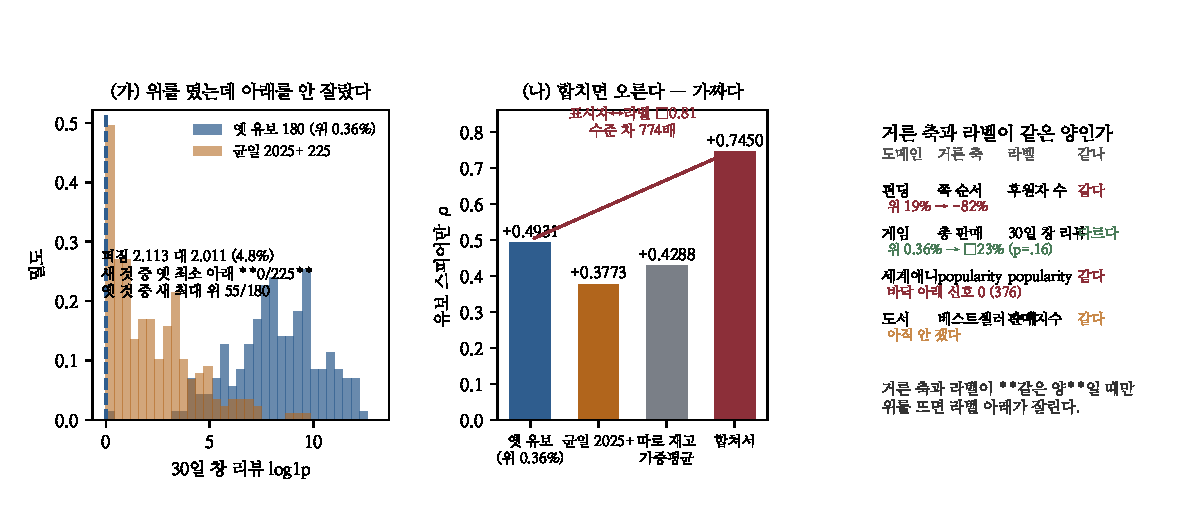
\includegraphics[width=\linewidth]{figs/fig384.pdf}
\caption{\textbf{(가)} 옛 유보와 균일 2025$+$의 라벨 분포. 퍼짐이 4.8\%
차이고 새 것 중 옛 최소 아래가 0개다. \textbf{(나)} 채점 방식별. 합치면
$+0.7450$ 로 \emph{오른다} --- 두 무리 수준 차가 774배라 표시자가 라벨과
$-0.80$ 이다. \textbf{(다)} 거른 축과 라벨이 같은 양인지로 네 도메인을
가른 표.}
\label{fig:main}
\end{figure}

\section{첫 수치를 안 채택했다}

\begin{center}
\begin{tabular}{lrrr}
\hline
무리 & 행 & 라벨 퍼짐 & $\rho$ \\
\hline
옛 유보 (위 0.36\%) & 180 & 2.113 & $+0.4931$ \\
균일 2025$+$ & 225 & 2.011 & $+0.3773$ \\
\hline
차 & & & $+0.1158$ \\
피셔 $z$ & & & $1.42$ ($p=0.155$) \\
\hline
\end{tabular}
\end{center}

27\% 떨어졌으니 ``게임도 부풀어 있었다''로 쓸 수 있었다. \textbf{그런데
$n=180$ 과 $225$ 로는 이 크기를 못 가른다.} 노트 133이 첫 양수를 그대로
채택하지 말라 한 자리이고, 이번에는 그 첫 양수가 \emph{내 예측과 같은
방향}이라 더 위험했다 --- 노트 382가 ``게임이 다음 펀딩''이라고 이미 써
놓았다.

\textbf{판정: 게임의 수집 편향이 도메인 점수를 부풀린다는 것은 확인되지
않았다.} 채택할 것도 없다(챔피언 그대로 판 0.4355 · 분모 3,430).

\section{왜 펀딩과 다른가}

\begin{center}
\begin{tabular}{lrr}
\hline
 & 펀딩 (노트 379) & 게임 (여기) \\
\hline
우리가 뜬 구역 & 위 19\% & 위 \textbf{0.36\%} \\
새 행 중 옛 바닥 아래 & 157/449 (35\%) & \textbf{0/225} \\
라벨 퍼짐 옛 대 새 & 0.407 대 0.621 & 2.113 대 2.011 \\
$\rho$ 옛 대 새 & $+0.3746 \to +0.0667$ & $+0.4931 \to +0.3773$ \\
 & (같은 구간에서도) & ($p=0.155$) \\
\hline
\end{tabular}
\end{center}

게임이 훨씬 좁게 뜬 표본인데 라벨 아래가 안 잘렸다. \textbf{거른 축과
라벨이 다른 양이기 때문이다.}

\begin{center}
\begin{tabular}{llll}
\hline
도메인 & 거른 축 & 라벨 & 같나 \\
\hline
펀딩 & 목록 쪽 순서 & 후원자 수 & 같다 \\
게임 & 총 판매(\texttt{topsellers}) & \textbf{30일 창} 리뷰 & \textbf{다르다} \\
세계애니 & popularity & popularity & 같다 \\
도서 & 베스트셀러 순위 & 판매지수 & 같다 \\
\hline
\end{tabular}
\end{center}

총 리뷰가 많은 게임 중에도 출시 30일에는 조용했던 것이 흔하다 --- 노트
210이 라벨을 총계에서 30일 창으로 바꿨을 때 노린 것이 바로 그 분리였고,
\textbf{그 고침이 수집 편향까지 덜어 주고 있었다.} 아무도 그 값으로
계산한 적은 없다.

\textbf{규칙으로 적는다: 수집 편향이 도메인 점수를 부풀리는 것은 거른
축과 라벨이 같은 양일 때다.} 다르면 위를 떠도 라벨 범위가 안 잘린다.
그러면 노트 375의 분류에 물어야 할 것이 하나 더 붙는다 --- ``잘렸나''
앞에 ``무엇으로 잘랐나''.

\section{반대 방향의 함정}

\begin{center}
\begin{tabular}{lrr}
\hline
채점 & 행 & $\rho$ \\
\hline
옛 유보만 & 180 & $+0.4931$ \\
균일만 & 225 & $+0.3773$ \\
따로 재고 가중평균 & 405 & $+0.4288$ \\
\textbf{합쳐서} & 405 & $\mathbf{+0.7450}$ \\
\hline
\end{tabular}
\end{center}

라벨 중앙이 3,872 대 5 로 774배라 ``어느 표본에서 왔나'' 표시자가
라벨과 $-0.8070$ 이고 예측과도 $-0.7153$ 이다. 모형은 상위 판매작이 신작
평균보다 크다는 것을 맞히고, 그 맞힘이 순위 상관을 통째로 부풀린다.

\textbf{그래서 ``대표 표본을 넣었더니 판이 올랐다''는 문장은 증거가
아니다.} 펀딩에서는 같은 편향이 점수를 내렸고 게임에서는 올린다. 노트
377이 팝업에서 찾은 계수 기준 표시자($+0.4416$)와 같은 기제인데
\textbf{부호가 반대}다.

\section{남은 것}

\begin{center}
\begin{tabular}{lll}
\hline
항목 & 왜 값이 큰가 & 어떻게 \\
\hline
도서 & 거른 축과 라벨이 같은 양이다 & 베스트셀러 밖 균일 표본 \\
게임 균일 $n$ 늘리기 & 141$\to$225 로도 $p$ 가 안 움직였다 & 500 이상 · 또는 다른 라벨 \\
게임 아래 25\% & 라벨 아래 4분위가 음수다 & 노트 376 절차로 따로 \\
30일 창 라벨 아홉으로 & 라벨을 바꾸면 편향이 준다 & 게임만 갖고 있다 \\
\hline
\end{tabular}
\end{center}

\end{document}
